\section{Setup client}You can see the list of clients that are ready for partitioning and formatting. These clients have completed the hardware detection sequence.\\
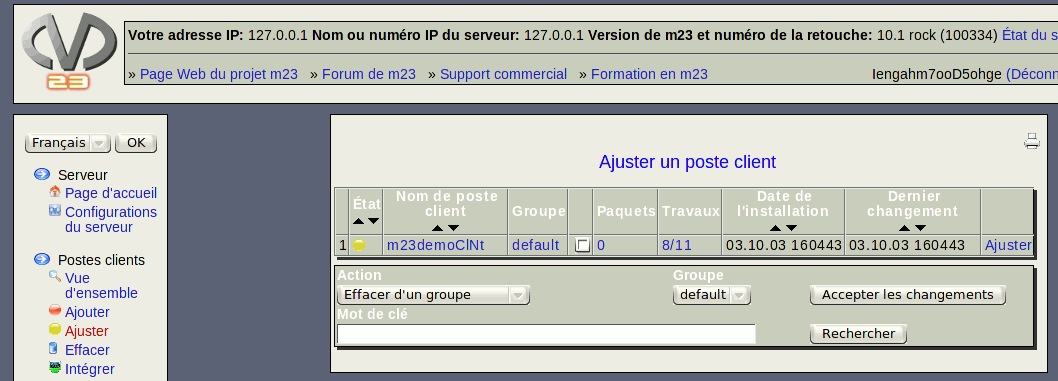
\includegraphics[scale=0.4]{/mdk/doc/manual/screenshots/en/clients_setup.png} \\
To partition and format the client click on \textit{"Setup"}.\\
If you click on the client name, you get detailed information about the selected client and can enter the control center.\\
\subsection{Status description}
The color marks the installation status of the client.\\
\begin{itemize}
\item \textbf{red}: Client is added, but hardware detection is not complete.\\
\item \textbf{yellow}: Now you can partition and format the client. A base system with graphical user interface is installed automatically.\\
\item \textbf{green}: The base system is installed, now you can add some additional software packages.\\
\item \textbf{blue}: Currently the client installs additional software.\\
\item \textbf{orange}: The client is in the \textbf{critical state}. That means there was an error during installation which must be solved by the administrator. The control center gives you some solution proposals to solve the critical state.\\
\item \textbf{white}: This is a master client for mass installation from whom the settings are transferred to the other clients.\\
\item \textbf{bug}: The bug indicates that the client is in debug mode.\\
\end{itemize}
\subsection{Jobs}
In this row you can see the amount of waiting jobs before and the amount of all jobs after the slash.\\
\subsection{Work on multiple clients}
Select the clients by checking the boxes in the client lines.\\
Now you can work on all selected clients::\\
\begin{itemize}
	\item \textbf{remove from group}: Select the group, all clients should be deleted from. Nothing is done, if a client is not in the selected group.\\
	\item \textbf{add to group}: Select the group, all clients should be added to. Nothing is done, if a client already is in the selected group.\\
	\item \textbf{Delete}: Deletes the selected clients.\\
\end{itemize}
\subsection{Hint}
Use the refresh function of your browser to see the current status of your clients. (e.g. by pressing the F5 key).\\
\subsection{Gimmicks}
\begin{itemize}
\item You can change the status of a client if you click on the according status symbol. You should only change the status if you know what you are doing.\\
\item The debug mode can be (de)activated by clicking the bug icon.\\
\end{itemize}
